%\PassOptionsToPackage{draft}{graphicx} 
\documentclass[11pt]{article}

\usepackage{sbc-template}

\usepackage{textcomp}
\usepackage{amsmath}
\usepackage{amsfonts}
\usepackage{amssymb}
\usepackage{url}
\usepackage{graphicx} 
\usepackage{bm}
\usepackage{listings}
\usepackage[usenames,dvipsnames]{color}
\usepackage[utf8]{inputenc} 
\usepackage[T1]{fontenc}    
\usepackage[english]{babel}     
\usepackage{lmodern}		

\usepackage{bm}

\textwidth 16cm
\textheight 22cm
\oddsidemargin 0cm
\evensidemargin 0cm
\topmargin -0.8cm

\newcommand{\tuple}[1]{\ensuremath{\left \langle #1 \right \rangle }}
\DeclareMathOperator*{\argmax}{arg\,max}

\definecolor{black}{RGB}{0,0,0}
\definecolor{gray}{RGB}{100,100,100}
\definecolor{light-gray}{RGB}{150,150,150}

\newcommand{\commandlisting}{
  \lstset{ %
  language=sh,                % the language of the code
  numbers=none,         % where to put the line-numbers
  tabsize=4,                      % sets default tabsize to 2 spaces
  breaklines=true,
  %basicstyle=\small\ttfamily,
  framerule=0pt,
  backgroundcolor=\color{GreenYellow}, % choose the background color. You must add \usepackage{color}
  columns=flexible,
  escapeinside={\#*}{*)},            % if you want to add a comment within your code
  breakatwhitespace=false,        % sets if automatic breaks should only happen at whitespace
  showtabs=false,                % show tabs within strings adding particular underscores
  upquote=true,
  showspaces=false,
  showstringspaces=false
  }
}

\newcommand{\outputlisting}{
  \lstset{ %
  language=sh,                % the language of the code
  numbers=none,         % where to put the line-numbers
  tabsize=4,                      % sets default tabsize to 2 spaces
  breaklines=true,
  basicstyle=\small\ttfamily,
  framerule=0pt,
  backgroundcolor=\color{light-gray}, % choose the background color. You must add \usepackage{color}
  columns=flexible,
  escapeinside={\#*}{*)},            % if you want to add a comment within your code
  breakatwhitespace=false,        % sets if automatic breaks should only happen at whitespace
  showtabs=false,                % show tabs within strings adding particular underscores
  upquote=true
  }
}

\newcommand{\mpilisting}{
  \lstset{ %
  language=c,                % the language of the code
  numbers=none,         % where to put the line-numbers
  tabsize=4,                      % sets default tabsize to 2 spaces
  breaklines=true,
  basicstyle=\small\ttfamily,
  framerule=0pt,
  backgroundcolor=\color{light-gray}, % choose the background color. You must add \usepackage{color}
  columns=flexible,
  escapeinside={\#*}{*)},            % if you want to add a comment within your code
  breakatwhitespace=false,        % sets if automatic breaks should only happen at whitespace
  showtabs=false,                % show tabs within strings adding particular underscores
  upquote=true,
  showspaces=false,
  showstringspaces=false
  }
}

%\large

\sloppy

\title{Virtualized Experiments for Scientific Parallel Applications (VESPA) - Installation Manual}

\author{Giacomo Victor Mc Evoy Valenzano\inst{1}}


\address{ComCiDis -- Laborat\'orio Nacional de Computa\c c\~ao Cient\'ifica (LNCC)
  \email{giacomo@lncc.br}
}

\begin{document} 

\maketitle

\section{Introduction} 

This document describes the installation process for the software system called Vespa (Virtualized Experiments for Scientific Parallel Applications). Vespa is designed to support the definition and production of controlled application executions running on virtual machines (VMs), as well as gathering performance metrics related to these executions. 
 
The main goal of Vespa is to manage the systematic experimentation of applications deployed on different virtual clusters, while supporting rich definitions for the cluster topology and mappings to underlying physical resources. The results will later translate into a knowledge repository with real (non-simulated) data for studying the effects of virtual cluster features on different scientific applications.

Vespa is not meant to be a tool for deploying applications in the Cloud or in virtualized environments. It is specifically aimed at improving the understanding of how virtualization affects application performance. While Vespa performs the deployment of the virtual cluster and the execution of the application, it does \textbf{not} currently configure the VMs (assumes the VM images are ready), \textbf{nor} does it takes care of the application deployment (assumes the application has an executable properly installed and ready to be called).

Reading the manual: 

\commandlisting
\begin{lstlisting}[caption={Example of command (auser@somehost)}]
issue this command in the console, possibly adapting variables
\end{lstlisting}

\outputlisting
\begin{lstlisting}[caption={Example of file contents / output}]
Either the required contents of a file, or an example of console output
\end{lstlisting}


\section{About Vespa}

\subsection{Definitions}

%Vespa is based on the following definitions and specifications.

\begin{description}
  \item [Virtual Cluster:] Aggregation of Virtual Machines inter-connected with a virtual network, supporting the execution of a parallel application. It is described by a \emph{Virtual Cluster Characterization}, see Figure \ref{fig:vcluster}.
  \item [Core Placement:] Representation of the spatio-temporal allocation of a virtual core, in terms of its mapping onto physical cores. 
  \item [Virtual Machine Placement:] Traditionally, it is defined as the selection of the hosting physical node for each given VM. Here, it is defined as an aggregation of \emph{Core Placement} instances for all the virtual cores of a VM.
  \item [Cluster Placement:] Defined as aggregation of the \emph{Virtual Machine Placement} instances for all the VMs of a \emph{Virtual Cluster}. Unambiguously describes how each virtual core in
  the cluster is mapped onto physical cores. Can be separated in \emph{Cluster Topology} and \emph{Physical Mappings}.
  \item [Cluster Topology:] Describes the arrangement of cores in the same way as a physical cluster, details of this description are visible to applications deployed inside the virtual cluster. 
  \item [Physical Mappings:] Correspond to details of the core placement that are not visible to applications deployed inside the virtual cluster, e.g. settings for pinning virtual cores to a subset of available physical cores.
  \item [Application:] A scientific benchmark, application or workflow element with execution in finite time.
  \item [Execution:] A single instance of an \emph{Application}, has start time and finish time.
  \item [Experiment:] Instantiation of a \emph{Virtual Cluster} followed by one or more sequential application \emph{Executions} on said \emph{Virtual Cluster}, includes the gathering of \emph{Performance Metrics}.
  \item [Scenario:] Orchestration of one or more concurrent \emph{Experiments}, includes the life-cycle management of the \emph{Virtual Clusters}. Currently, Vespa supports the definition of concurrent \emph{Experiments}, but not the actual execution. %captures the spatio-temporal distribution of the \emph{Experiments}.
  \item [Performance Metrics:] Relevant generated data about \emph{Experiments}. Classified as scalar metrics (single value for each \emph{Execution}) and temporal metrics (time series for each \emph{Execution}). Also classified as system metrics (CPU, memory, network utilization) and application metrics (runtime, application-specific throughput).
\end{description}

\begin{figure}[h!]
\centering
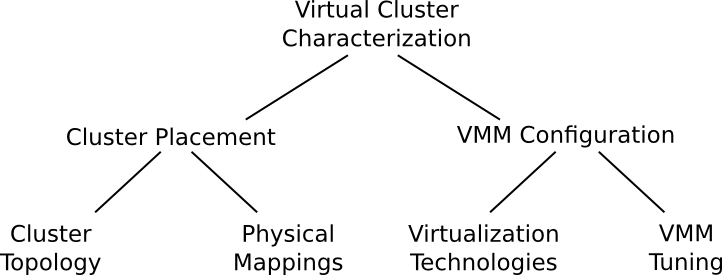
\includegraphics[scale=1.0]{figures/vcluster.png} 
\caption{Hierarchical view of proposed characteristics of a virtual cluster.}
\label{fig:vcluster}
\end{figure}

\subsection{Assumptions and Limitations}

\begin{enumerate}
  \item Applications consist of a variable set of processes, which are deployed in one or more VMs on execution. Each VM hosts processes corresponding to a single application.
  \item Processes of a given application are either equal (SPMD approach) or reflect the Master/Worker paradigm. A process may not migrated to other VMs once it starts execution.%, but a VM may be migrated to a different host at runtime.
  \item Vespa currently assumes a homogeneous physical environment, but this assumption may be relaxed in the future.
  \item Vespa currently supports virtual clusters composed of homogeneous VMs, but this limitation may be relaxed in the future.
  \item Vespa currently uses a simplified characterization of the \emph{Virtual Cluster Placement} based on four primary variables and two secondary variables:
  \begin{itemize}
    \item \textbf{Number of cores (\texttt{nc}):} the total number of virtual cores deployed in the cluster. Assuming that each application process will be assigned to one virtual core, this matches the total number of processes \textit{np}.
  \item \textbf{Number of cores per VM (\texttt{cpv}):} the number of virtual cores for each VM, held constant for a virtual cluster, due to item 4. 
  \item \textbf{Distribution factor (\texttt{df}):} a value ($df \in [0, 1]$) that measures the consolidation or scattering of the VMs along physical machines. Let $vpm$ be the total number of virtual cores executing on each PM, \texttt{df} is thus given by
\begin{equation}
\label{eq:df}
df = \left\{
  \begin{array}{ll}
    0         & \textrm{if } vpm=nc \\
    \frac{1}{vpm}   & \textrm{otherwise}
  \end{array}
  \right.
\end{equation}

  Let $ppm$ be the total number of physical cores in every PM, a value of $df=1/ppm$ thus indicates that the VMs are consolidated in as few physical machines as possible, unless the virtual cluster is deployed in a single physical machine, which is denoted as $df=0$. %A value of $df=1$ indicates that the VMs have a single core each and have maximum spread over the PMs. This definition enables comparison between deployments under different physical topologies.

  \item \textbf{Pinning strategy (\texttt{pstrat}):} the scheme used to map virtual cores to physical cores. By default, all physical cores in a PM are eligible to execute processes assigned to a virtual core, but it is possible to specify a subset of physical cores that are eligible. Five pinning strategies are currently available, called \texttt{NONE}, \texttt{GREEDY}, \texttt{BAL-ONE}, \texttt{BAL-SET} and \texttt{SPLIT}. 
  \end{itemize}

  \item \textbf{Two secondary variables:} \texttt{deployedNodes}, which specifies the identities of the PMs that are hosting VMs for the virtual cluster; \texttt{deployedSockets}, which specifies the identities of the eligible processor sockets, which in turn affect the identities of resulting physical cores $\tuple{p}_i$ for each virtual core $v_i$. On non-concurrent experiments, these variables can assume default values (first physical nodes and all physical sockets).

  \item The current representation of generated data supports only scenarios with single \emph{Executions} (without concurrency). 


%\item Resource consumption of a VM is dependent on the spatial distribution of other collaborating VMs.
%\item Process performance can be affected by resource consumption of other VMs in the same host. %(resource contention).
%\item At any given time, each virtual core can be assigned to a subset of the physical cores inside the host, via the virtual core mapping.  
\end{enumerate}

\subsection{Features of Vespa}

%\subsection{Functionality Elements}

\begin{itemize}
  \item \textbf{Defining Experiments:} The Scenarios that are supported by Vespa are described in an Experiment Definition File, it is the main input for running experiments. Vespa provides a module for creating the file according to different parameters. The module's arguments are used to specify ranges for sweeping parameters such as virtual cluster size, distribution, pinning strategy, etc. 

  \item \textbf{Running Experiments:} The main function of Vespa is to execute parallel applications on virtual clusters. These executions are described in the Experiment Definition File, and are orchestrated in sequence and independently. For each scenario, the necessary \emph{Virtual Clusters} are created, the \emph{Applications} are executed a number of times (runs), the performance metrics are gathered, and the Virtual Clusters are destroyed. This sequential process is automated as to not require human intervention.

\begin{figure}
\centering
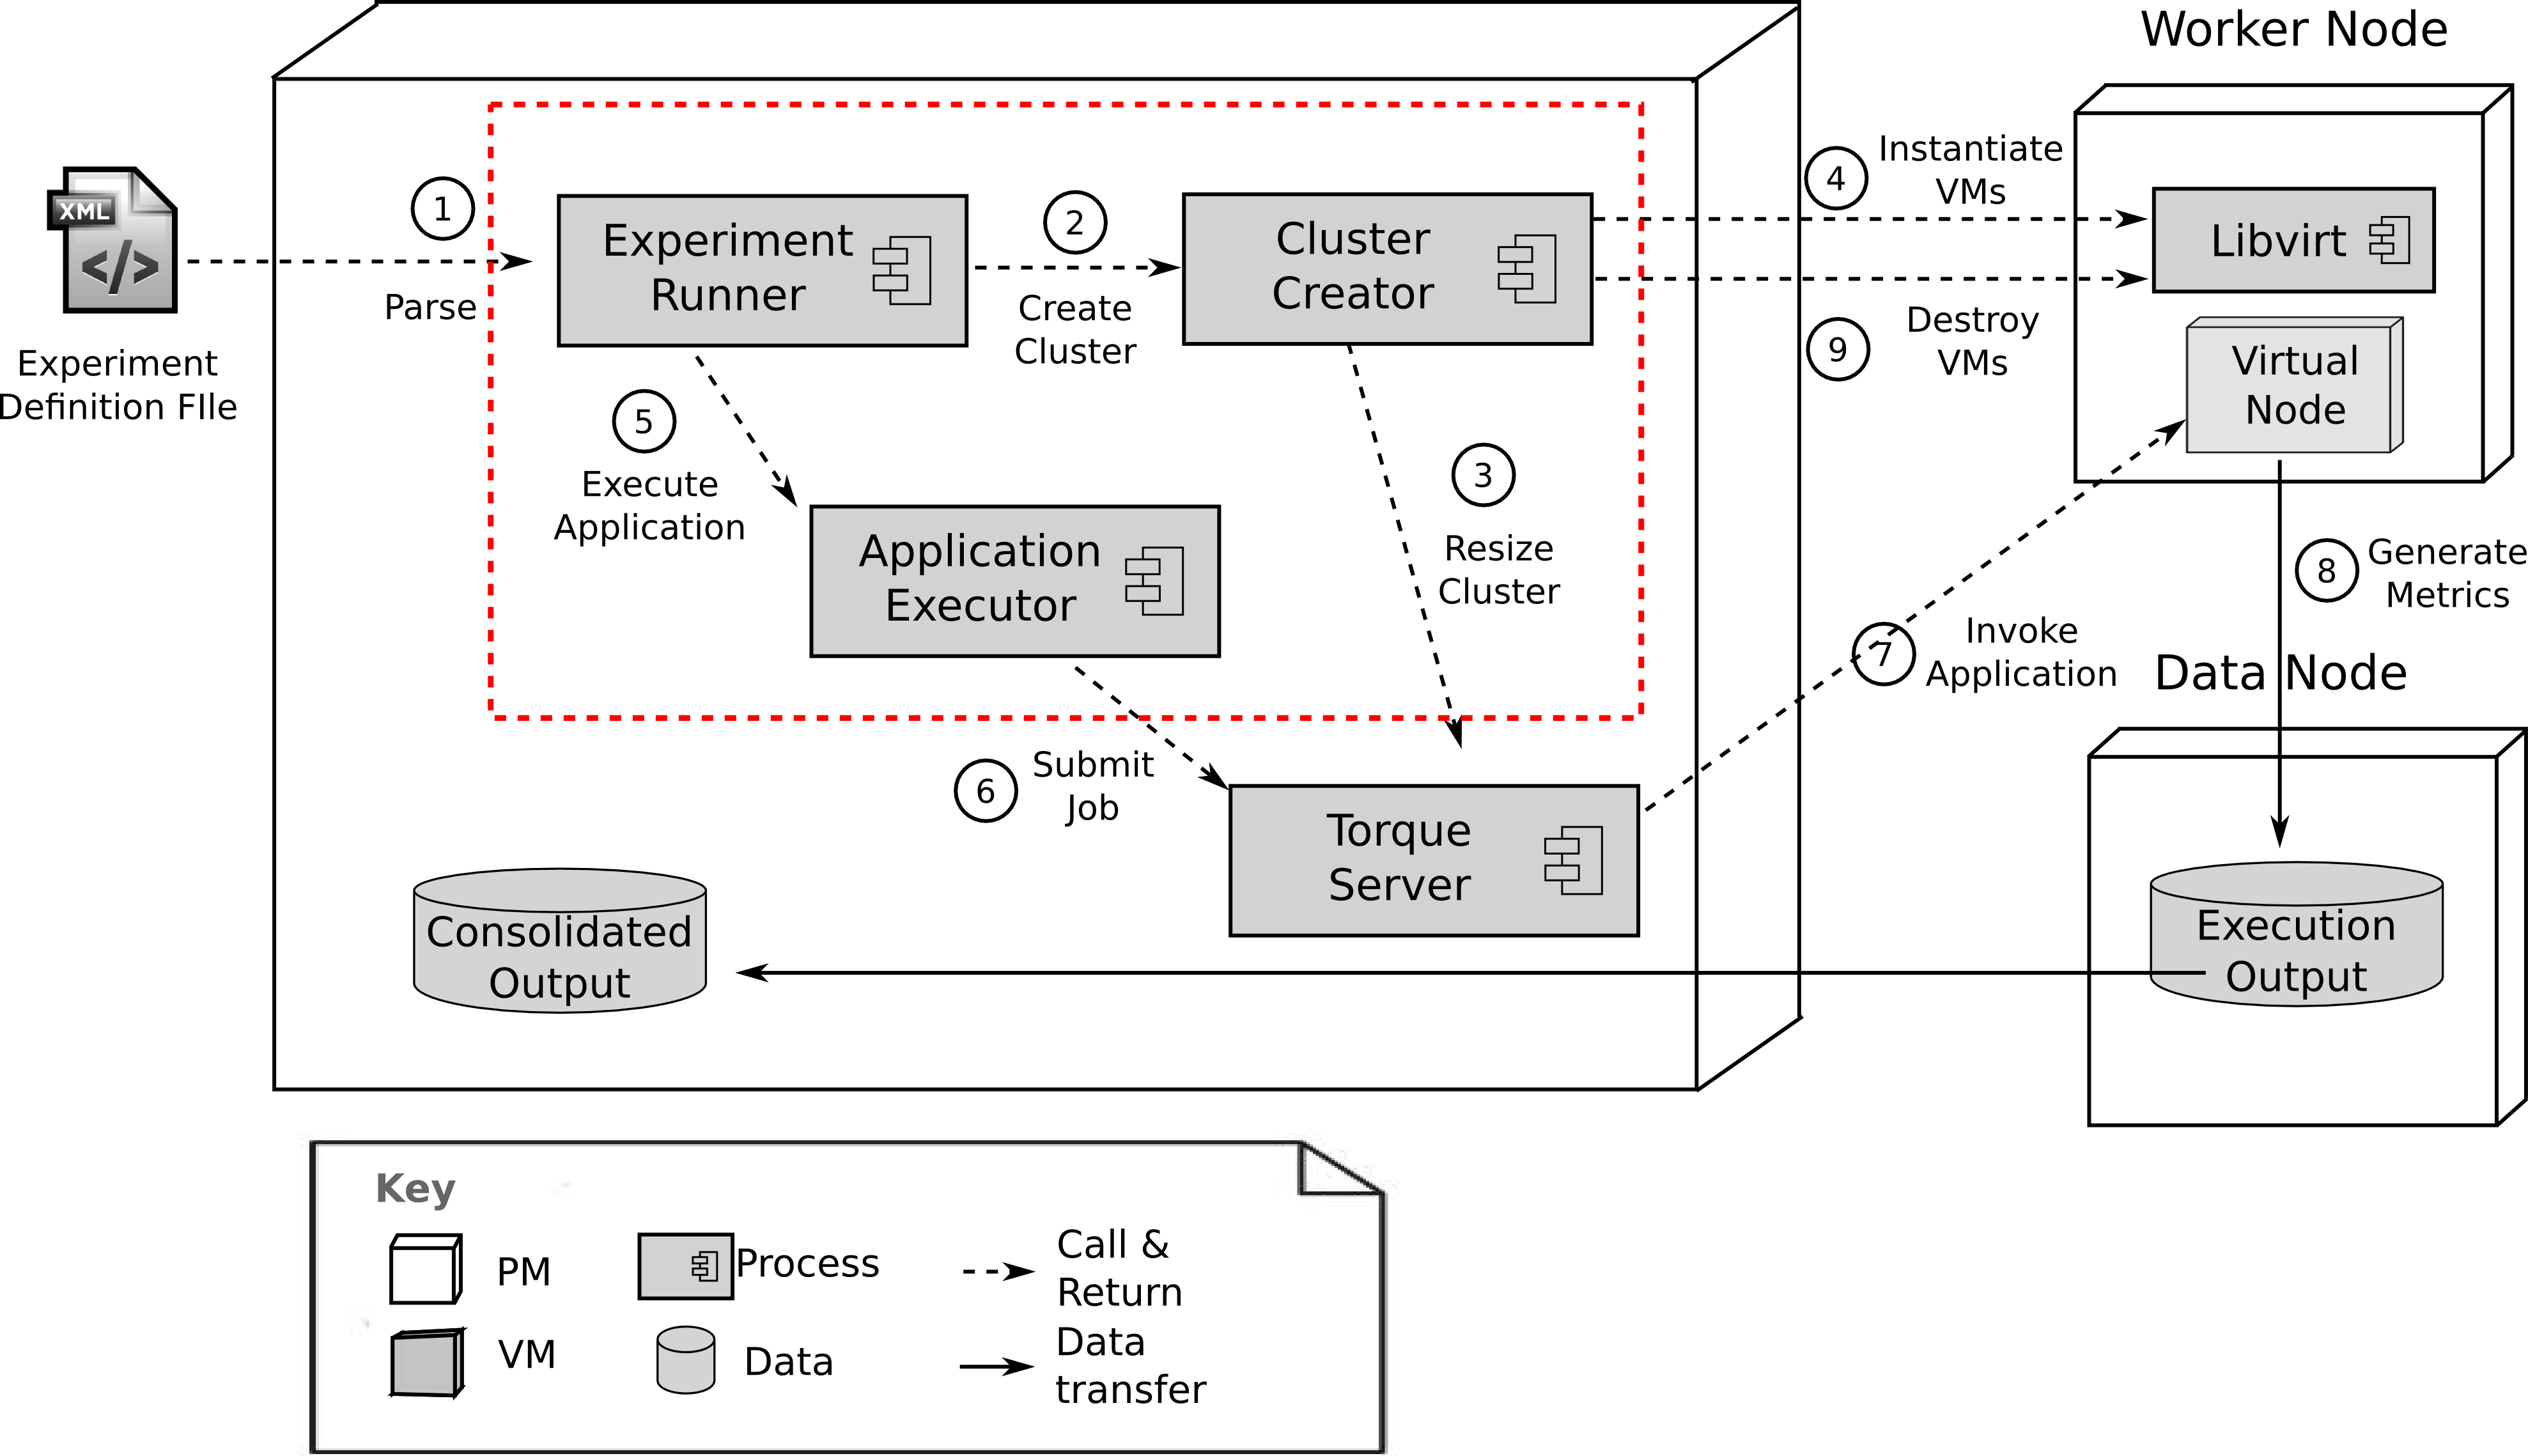
\includegraphics[scale=0.38]{figures/execution.png}
\caption{Deployment and execution view for Vespa architecture.}
\label{fig:Vespa}
\end{figure}

Vespa leverages the \emph{libvirt} virtualization library to manage the life-cycle of VMs remotely, and the \emph{PBS}-based, \emph{Torque} cluster manager to submit executions to the virtual cluster. It is written in both shell script and the Python programming language. Before running any experiment, a master XML must be created as a VM definition template for \emph{libvirt}, as well as a master \emph{PBS} file for job submission, based both on customizable parameters. Furthermore, up to $ppm$ VM images are cloned in each PM, since at most $ppm$ VM instances will be hosted per PM. %$(when $cpv=1$).

Figure \ref{fig:Vespa} depicts a deployment diagram that shows the sequence to execute a Scenario using Vespa. The sequence is explained as follows:
\begin{enumerate}
  \item The Experiment Definition File is parsed. Besides stating the application and the number of executions, an experiment describes the characteristics of a virtual cluster as a composition of \emph{Cluster Placement} and \emph{VMM Configuration}. %, as well as the \emph{Torque} file used to submit the application on the virtual cluster.
  \vskip5pt
  \item The experiment input is used to calculate and generate the VM profiles required for the virtual cluster.
  \vskip5pt
  \item Since the \texttt{cpv} value can change between experiments, the \emph{Cluster Topology} needs to be redefined at the virtual head. Thus, the cluster description is updated in \emph{Torque} and the server daemon is restarted.
  \vskip5pt
  \item The generated VM profiles are used to instantiate the required working nodes in the virtual cluster. Vespa then waits for the VMs to be ready using \texttt{qnodes} command.
  \vskip5pt
  \item A component called Application Executor will generate the \emph{PBS} file used to submit the application on the virtual cluster.
  \vskip5pt
  \item The \emph{PBS} job is submitted to the \emph{Torque} server. Since Vespa uses the virtual cluster exclusively and topology matches request by design, execution can begin immediately.
  \vskip5pt
  \item The parallel application runs on the virtual nodes. During each execution, resource utilization of VMs and PMs can be monitored using the \texttt{sysstat} tool.
  \vskip5pt
  \item Each time the application completes an execution, performance data is generated by collecting \emph{sysstat} output and application-specific output.
  \vskip5pt
  \item Vespa queries Torque for job termination using the \texttt{qstat} command. When all executions finish, the working nodes of the virtual cluster are destroyed. The system returns to the initial state, and a new experiment can begin.
\end{enumerate}
  

  \item \textbf{Gathering of Performance Metrics:} Vespa currently uses the \texttt{sysstat} software to monitor both the virtual and physical environment during each \emph{Execution}. With \texttt{sysstat}, the utilization rate of CPU, memory and network is captured as time series that span the duration of the \emph{Execution}. The number of data elements retrieved depends on the \emph{Virtual Cluster Placement}, both its topology (number of VMs) and physical mappings (number of hosts). Vespa also registers the output of the \texttt{time} command, that informs the \texttt{userTime, systemTime} and \texttt{ellapsedTime}. Finally, an application-specific plugin may be configured for Vespa so that it captures an application metric such as throughput, e.g. a \emph{Gflops} metric for each \emph{Execution}.

  \item \textbf{Consolidation of Performance Metrics:} At any time, the user may be interested in producing a consolidated performance report for an application. A Vespa module is used to produce a folder and two CSV files that include all the aforementioned metrics.  
\end{itemize}

\section{Vespa Setup}
\label{sec:setup}

This section describes the procedure needed for setting up Vespa to a usable state. It consists of steps needed to create the virtual network, deploy the VMs and configure an execution environment for the applications.

\subsection{Getting Vespa}

The code for Vespa is currently available at: \url{https://github.com/ginomcevoy/vespa}

\subsection{Physical Environment}

The physical cluster comprises a head node of the cluster (referred to as \textit{head}) and one or more computing nodes for the instantiation of VMs (referred to as \textit{nodes}). 

The preferred network topology is presented in Figure \ref{fig:phynet}. The B-class subnet (172.16.X.X) is preferred because it allows for more than 255 machines (physical and virtual) in the same network. Using the B-class, the IP addresses are organized so that the 172.16.1.X addresses (physical machine and the VMs hosted in it) correspond to the first node, the 172.16.2.X addresses to the second node, and so on. In this example, each node has the 172.16.X.254 address. Default Vespa configuration assumes that the first addresses of the 172.16.X.0 subnet will be used for the VMs.

\begin{figure}[h!]
\centering
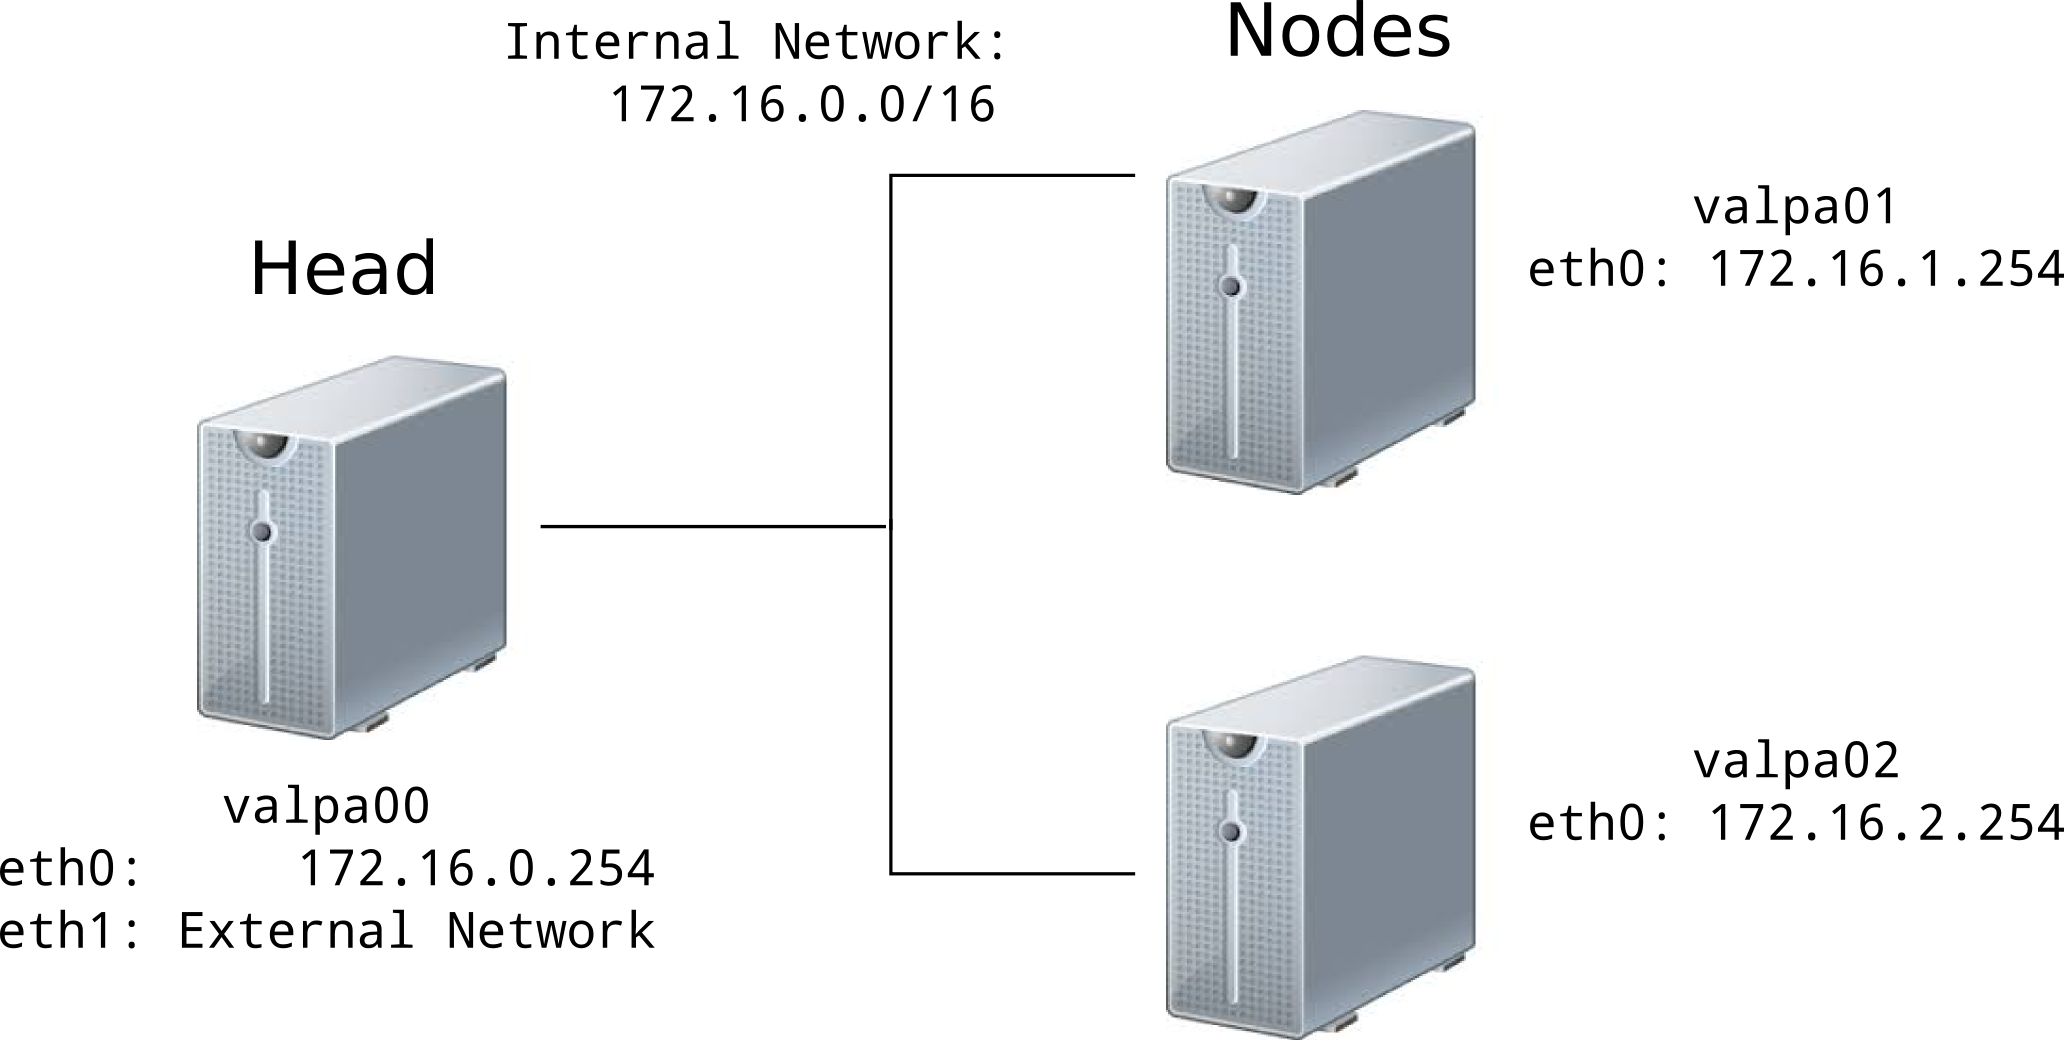
\includegraphics[scale=0.75]{figures/phynet.png}
\label{fig:phynet}
\caption{Topology of the physical cluster (head and nodes).}
\end{figure}

The Vespa software should be placed in the \textit{head} filesystem (ex. \texttt{/home/vespauser/vespa}). This directory will be known as \texttt{VESPA\_HOME}. The scripts will automatically execute using relative paths. The Operating System (OS) used to show the procedure is Ubuntu 14.04 64 bits. The dependencies are then met as follows:

\commandlisting
\begin{lstlisting}[caption={Vespa package dependencies (vespauser@head)}]
sudo apt-get install libvirt-bin qemu-kvm bridge-utils torque-client \
python-setuptools pip virt-viewer virtinst openssh-server parallel
\end{lstlisting} 

\commandlisting
\begin{lstlisting}[caption={Vespa package dependencies (vespauser@nodes)}]
sudo apt-get install libvirt-bin qemu-kvm bridge-utils openssh-server sysstat
\end{lstlisting}

In order to test the libvirt installation, connect using \texttt{virsh} command:

\outputlisting
\begin{lstlisting}[caption={Libvirt test (vespauser@head)}]
$ virsh list
 Id Name                 State
----------------------------------

\end{lstlisting}

Vespa relies on the \texttt{Ansible} configuration management tool. While it is available through apt-get \texttt{quik} python package, Vespa requires version 0.9+:

\commandlisting
\begin{lstlisting}[caption={Installing Ansible (vespauser@head)}]
sudo pip install ansible
\end{lstlisting}

For Vespa to function, password-less SSH is needed between the head and the nodes. The easiest way to achieve this is to generate a SSH key and copying it to all nodes. To create the SSH key:

\commandlisting
\begin{lstlisting}[caption={SSH key (vespauser@head)}]
ssh-keygen -t rsa
cat ~/.ssh/id_rsa.pub >> ~/.ssh/authorized_keys
\end{lstlisting}

The key (private and public components, \texttt{id\_rsa id\_rsa.pub}) should be \textbf{sent via SSH} (manually) to the other nodes. Once copied, the following commands will both install the same key in a node, as well as registering the key for password-less SSH:

\commandlisting
\begin{lstlisting}[caption={SSH key (each node)}, label={lst:sshnode}]
mkdir ~/.ssh
cp id_rsa id_rsa.pub ~/.ssh
cat ~/.ssh/id_rsa.pub >> ~/.ssh/authorized_keys
\end{lstlisting}

Vespa expects the file \texttt{config/vespa.nodes} to be populated with the node names. In the following example, 12 physical nodes are available to Vespa:

\outputlisting
\begin{lstlisting}[caption={Example for config/vespa.nodes}]
# This file is the initial inventory file in INI format.
# It is read by Vespa to find define the computing nodes.
# Write the hostnames of each computing node here, one per line.
valpa01
valpa02
valpa03
\end{lstlisting}

The file \texttt{VESPA\_HOME/config/hardware.params} contains configuration parameters related to the physical environment, and \textbf{should be edited accordingly for correct Vespa setup}:

\outputlisting
\begin{lstlisting}[caption={Example for config/hardware.params}]
[Hardware]
# number of cores per node
cores=12
# number of processors (sockets) per node
sockets=2
# memory per node (GB)
mem=24
\end{lstlisting}

This file is read automatically by Vespa when executing either a shell or python script. With this configuration, it is possible to use the \texttt{VESPA\_HOME/mgmt-nodes/cluster-ssh.sh} script in order to send commands to all the nodes via SSH. The same folder includes similar scripts for managing the physical cluster.

\commandlisting
\begin{lstlisting}[caption={Usage of VESPA\_HOME/mgmt-nodes/cluster-ssh.sh (vespauser@head)}]
./cluster-ssh.sh <command to be executed on nodes via SSH>
\end{lstlisting}

\outputlisting
\begin{lstlisting}[caption={Example of VESPA\_HOME/mgmt-nodes/cluster-ssh.sh (vespauser@head)}]
$ ./cluster-ssh.sh hostname
valpa01 | success | rc=0 >>
valpa01

valpa02 | success | rc=0 >>
valpa02

valpa03 | success | rc=0 >>
valpa03
\end{lstlisting}

\subsection{Setting up the Virtual Network}

The file \texttt{config/vespa.params} handles most of the configuration parameters for VESPA. Here is the relevant section for configuring the virtual network (only showing B-class parameters):

\outputlisting
\begin{lstlisting}[caption={config/vespa.params (Networking)}]
###############################################################################
# Main networking option: one of {libvirt-bridge | external-bridge | sriov}
###############################################################################
# Vespa will use this value when creating the VM definitions.
# ALL options imply a virtual network created in libvirt for each physical node
# The setup/define-virtual-networks.sh script can be used to generate the XML
# definitions for these networks
# 
# libvirt-bridge:   instructs Vespa to use a bridge managed by libvirt
#         (DHCP by libvirt)
# external-bridge:  instructs Vespa to use a previously defined bridge 
#         (bridge and DHCP external to libvirt)
# sriov:          instructs Vespa to use the Virtual Functions of a 
#         SR-IOV network
network_source=external-bridge
\end{lstlisting}

The default \texttt{network\_source=external-bridge} relies on external configuration of the virtual bridges. Choosing \texttt{network\_source=libvirt-bridge} will instruct Vespa to manage the virtual bridges using \textit{libvirt}, see Appendix A. In any case, the configuration file \textbf{does not need to be modified} in order to get virtual clusters in the B-class IP address range.

For the purposes of this manual, the \texttt{network\_source=external-bridge} option is preferred. What follows is then the manual configuration of the virtual bridges and the DHCP server.

\subsubsection{Setting up the virtual bridges}

In each physical node, edit the \texttt{/etc/networking/interfaces} file for the virtual bridge. The example that follows corresponds to a class B network for the node \texttt{vespa01} (172.16.1.254).

\outputlisting
\begin{lstlisting}[caption={interfaces file (root@valpa01)}]
auto lo
iface lo inet loopback

auto eth0
iface eth0 inet manual

auto br0
iface br0 inet static
  address 172.16.1.254
  network 172.16.0.0
  netmask 255.255.0.0
  broadcast 172.16.0.0
  gateway 172.16.0.254
  bridge_ports eth0
  bridge_stp off
  bridge_fd 0
  bridge_maxwait 0
\end{lstlisting}

In order for the bridge to become active, the node can be restarted:

\commandlisting
\begin{lstlisting}[caption={reboot (root@nodes)}]
reboot
\end{lstlisting}

\subsubsection{Configuring the DHCP server}

This section assumes that the DHCP server will listen to the eth0 interface of the head server. Install the Ubuntu package:

\commandlisting
\begin{lstlisting}[caption={Install DHCP package (vespauser@head)}]
sudo apt-get install isc-dhcp-server
\end{lstlisting}

The script at \texttt{VESPA\_HOME/networking/dhcpd-conf-builder.sh} can be used to generate a suitable \texttt{dhcpd.conf} file. After executing the script, review the output file at \texttt{VESPA\_HOME/data-output/dhcpd.conf} for adjustments.

\commandlisting
\begin{lstlisting}[caption={Create the dhcpd.conf file (vespauser@head)}]
VESPA_HOME/networking$ ./dhcpd-conf-builder.sh
\end{lstlisting}

Finish configuration of the DHCP server:

\commandlisting
\begin{lstlisting}[caption={Update DHCP configuration (vespauser@head)}]
sudo cp $VESPA_HOME/data-output/dhcpd.conf /etc/dhcp3/
sudo service isc-dhcp-server restart
\end{lstlisting}

\subsubsection{Updating /etc/hosts to resolve hostnames}

At this point, the physical nodes will have their final IP addresses. The following command will generate the entries for both the physical and virtual IP addresses at the specified output. These entries should be used to update the \texttt{/etc/hosts} file of the physical nodes.

\commandlisting
\begin{lstlisting}[caption={Creating /etc/host entries (vespauser@head)}]
VESPA_HOME/vespa$ python -m network.etchosts <output>
\end{lstlisting}
 
\subsubsection{Replicating Vespa files to physical nodes}

The physical nodes require VESPA's \texttt{monitor} module for monitoring the consumption of physical resources. With the \texttt{VESPA\_HOME/setup/send-vespa-nodes.sh}, this module is sent to the physical nodes, along with other support scripts.

\commandlisting
\begin{lstlisting}[caption={Sending Vespa modules to nodes (vespauser@head)}]
VESPA_HOME/setup$ ./send-vespa-nodes.sh
\end{lstlisting}

\subsubsection{Using vhost module (optional)}

By default, Vespa relies on the \texttt{vhost\_net} module in an attempt to improve inter-VM communication. This module should be loaded in the physical nodes. The following command loads the module immediately:

\commandlisting
\begin{lstlisting}[caption={Loading vhost module (root@nodes)}]
sudo modprobe vhost_net experimental_zcopytx=1
\end{lstlisting}

To persist the change after reboot, edit the \texttt{/etc/modprobe.d/vhost-net.conf} file:

\outputlisting
\begin{lstlisting}[caption={/etc/modprobe.d/vhost-net.conf}]
options vhost_net experimental_zcopytx=1
\end{lstlisting}

Vespa will automatically try to use \texttt{vhost} if available, else it will use the \texttt{virtIO} implementation from KVM. This fallback behavior is ensured by \texttt{libvirt}.

\subsubsection{Final setting}

Figure \ref{fig:phynet2} shows the final setting for the physical network. The bridges will host the virtual networks. With this configuration, all nodes will be able to reach all VMs.

\begin{figure}[h!]
\centering
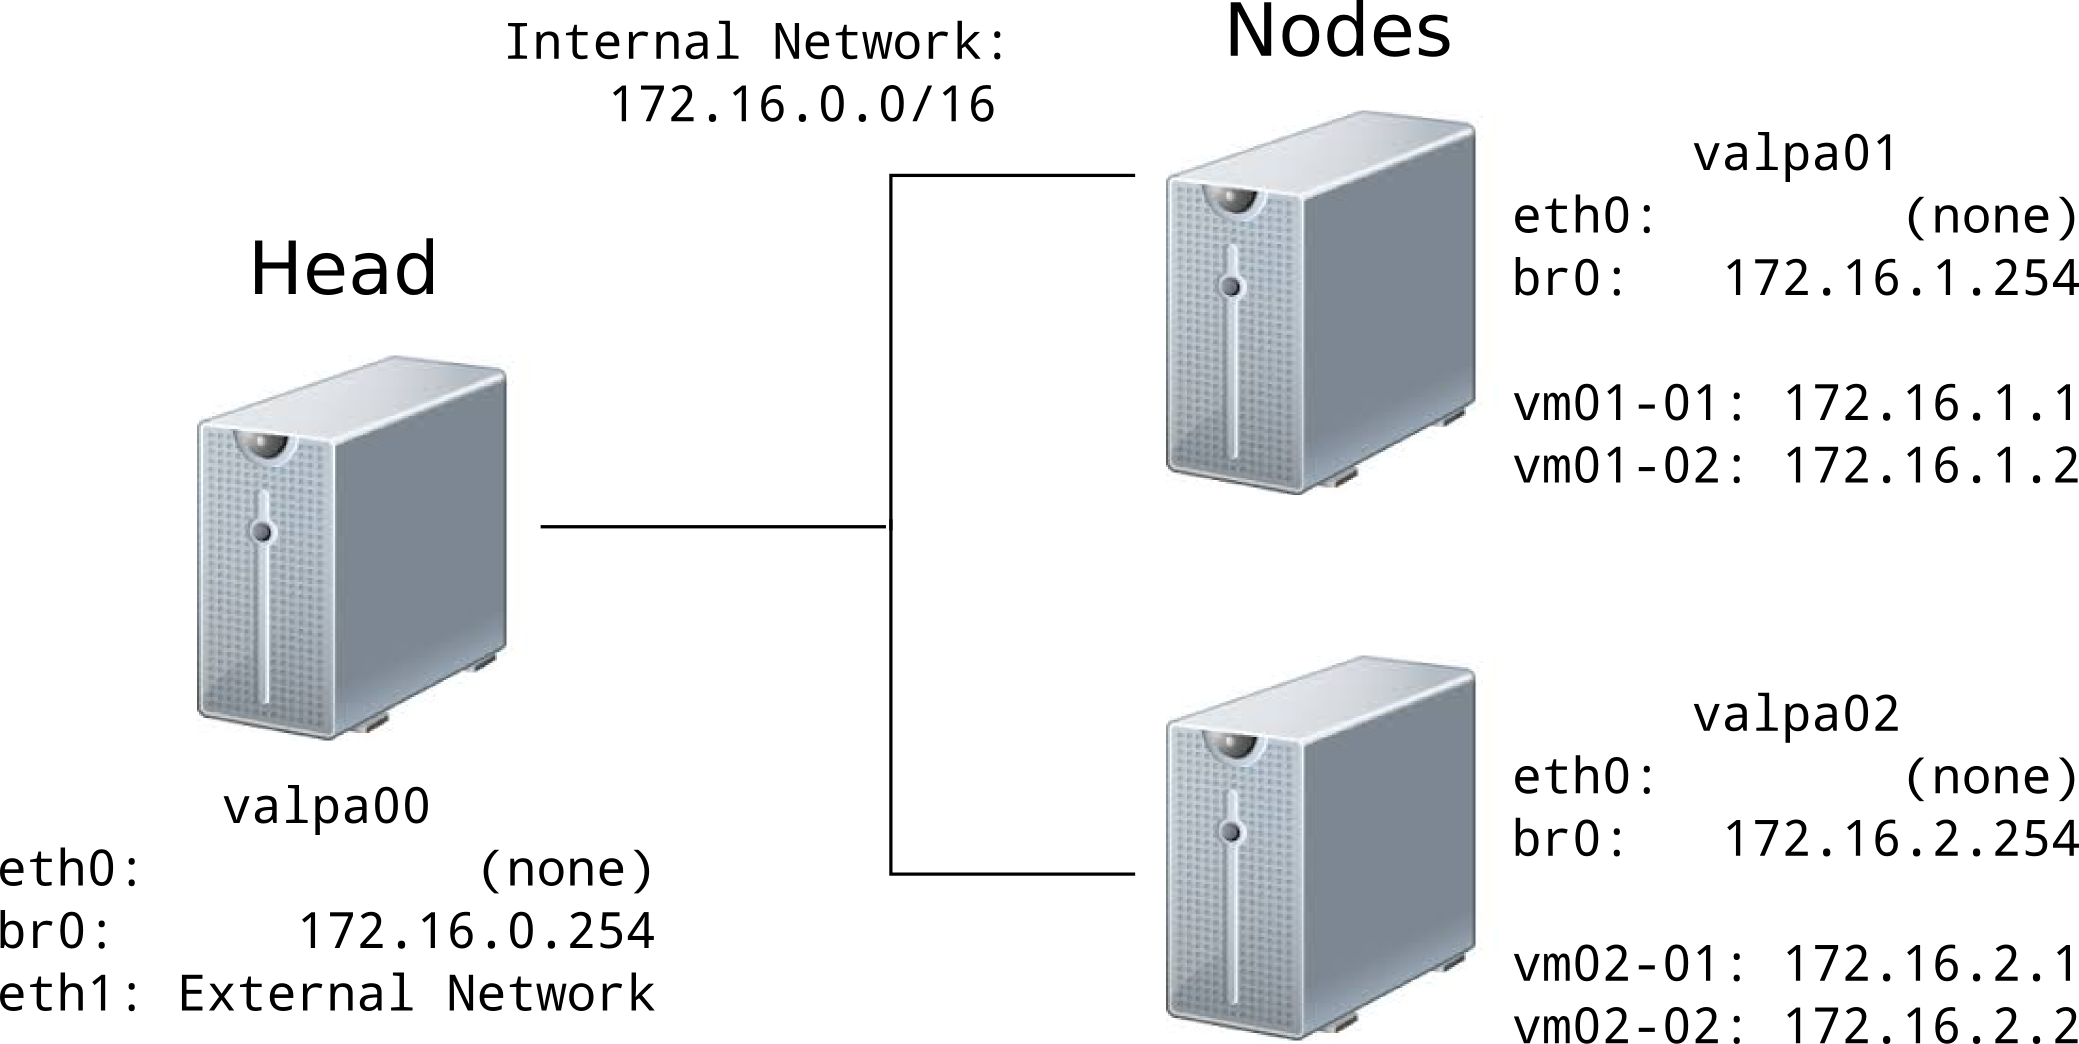
\includegraphics[scale=0.75]{figures/phynet2.png}
\label{fig:phynet2}
\caption{Topology of the physical cluster after creating the virtual bridges.}
\end{figure}

\subsection{Creating a VM}

Vespa requires the VM images used in the experiments to be created and deployed in advance. This requires having up to $ppn$ VM images in each node, where $ppn$ is the number of physical cores per node. The preferred way to deploy these images is to have a single master image in the head node, and create multiple copies of this image in the computing nodes.

To create a VM image, the \texttt{virt-install} command may be used to install a new OS (assuming Ubuntu 14.04). This requires access to the graphical capabilities of the head node, e.g. connecting using \texttt{ssh -X}. When installing the OS, the same username should be added (e.g. \texttt{vespauser}), and the \texttt{openssh-server} package should be added to gain SSH access to the node. The command is used as follows:

\commandlisting
\begin{lstlisting}[caption={Creating the first VM image (vespauser@head)}]
UBUNTU_ISO=<path to ISO installer>
MASTER_IMAGE_PATH=<path to master VM image>
virt-install --connect qemu:///system -r 512 -n vespa-vm -c $UBUNTU_ISO --disk path=$MASTER_IMAGE_PATH/disk.img --vnc --keymap=en-us
\end{lstlisting}

The \texttt{MASTER\_IMAGE\_PATH} path should have a base path for all VM images and a specific directory for the master VM image. The paths should be declared in \texttt{vespa.params} as well for later use:

\outputlisting
\begin{lstlisting}[caption={caption={params.sh (VM images)}}]
VM_IMAGE_PATH=~/vms                     # Path for all VM images
VM_IMAGE_MASTER=ubuntu14.04-node        # Specific path for master image 
DISK_FILENAME=disk.img     
\end{lstlisting}

At this point, the \textbf{SSH keys} of the head should be copied to the VM manually for password-less SSH (vespauser and root) with a procedure similar to Listing \ref{lst:sshnode}. Also, the \texttt{/etc/hosts} file needs to be \textbf{updated} using the entries from the \texttt{VESPA\_HOME/data-output/hosts} at the head.

(Remove /etc/udev/rules.d/70-persistent-net.rules)
(Set GRUB\_RECORDFAIL\_TIMEOUT=0 in /etc/default/grub)

\subsection{Setting up NFS}

Most distributed applications require a shared filesystem in order to aggregate results. In this manual, the NFS solution is used. The NFS server is installed in the head node, and the VMs will run NFS clients. The nodes may also run NFS clients to facilitate deployment. 

\commandlisting
\begin{lstlisting}[caption={Installing NFS server (vespauser@head)}]
sudo apt-get install nfs-kernel-server
\end{lstlisting}

A folder in the head node must be chosen to be exported to the clients, e.g. \texttt{/home/vespauser/shared}. The server is configured editing the \texttt{/etc/exports} file. The network must match the Vespa network (172.16.0.0/16 in this manual)

\outputlisting
\begin{lstlisting}[caption={Relevant section of /etc/exports (head)}]
/home/vespauser/shared  172.16.0.0/16(rw,sync,no_root_squash,no_subtree_check)
\end{lstlisting}

After creating the shared directory, activate the export:

\commandlisting
\begin{lstlisting}[caption={Activating NFS export (vespauser@head)}]
sudo exportfs -ra
\end{lstlisting}

The NFS clients should point to the server when mounting the shared folder. A permanent solution is to use an entry in \texttt{/etc/fstab}. Assuming preferred network configuration:

\outputlisting
\begin{lstlisting}[caption={Relevant section of /etc/fstab (Master VM)}]
# NFS
172.16.100.254:/home/vespauser/shared   /home/vespauser/shared   nfs  rsize=8192,wsize=8192,timeo=14,intr
\end{lstlisting}

The NFS client needs the appropriate package. Also, it may be necessary to start the mount manually:

\commandlisting
\begin{lstlisting}[caption={For mounting (Master VM)}]
sudo apt-get -y install nfs-common
sudo mount -a
\end{lstlisting}

In order for the mount to work, the folder \texttt{/home/vespauser/shared} must exist at the client. To ensure read/write access, the UID and GID of the user at the VM must match with the UID and GID of the user at the server. This can be enforced with the following commands (see \texttt{/etc/group} at the server for the correct values):

\commandlisting
\begin{lstlisting}[caption={Ensuring UID and GID (root@vm)}]
sudo apt-get install id-utils
sudo groupadd <groupname> --gid <GID>
sudo usermod --uid <UID> --gid <GID> vespauser
\end{lstlisting}

To test the permissions of NFS sharing, create a directory in \texttt{/home/vespauser/shared/} at the head node, and attempt to create a file within the directory using the VM console.

\subsection{Setting up Torque}

Vespa leverages the \emph{PBS}-based, \emph{Torque} cluster manager to submit executions to the virtual cluster. At the current stage of development, a single Torque server should be installed at the head node. This setting allows the instantiation of a single virtual cluster. Vespa will be later enhanced to support many concurrent virtual clusters with the same VM size, which can be supported with a single Torque server. Concurrent virtual clusters with different topologies require multiple Torque servers.

\subsubsection{Torque server (vespauser@head)}

To install the Torque server at the head node:

\commandlisting
\begin{lstlisting}[caption={Installing Torque server (vespauser@head)}]
sudo apt-get install torque-server torque-scheduler torque-client
\end{lstlisting}

Declare server name, must match hostname (using vespa00 as head)

\commandlisting
\begin{lstlisting}[caption={Torque server name (root@head)}]
echo vespa00 >> /var/spool/torque/server_name
\end{lstlisting}

Configure a default queue, and other configuration to ensure immediate execution

\commandlisting
\begin{lstlisting}[caption={Torque server queue (root@head)}]
qmgr -c "create queue batch queue_type=execution"
qmgr -c "set queue batch started=true"
qmgr -c "set queue batch enabled=true"
qmgr -c "set queue batch resources_default.nodes=1"
qmgr -c "set queue batch resources_default.walltime=3600"
qmgr -c "set queue batch max_running = 8"
qmgr -c "set queue batch resources_max.ncpus = 144"
qmgr -c "set queue batch resources_min.ncpus = 1"
qmgr -c "set queue batch resources_max.nodes = 144"
qmgr -c "set queue batch resources_default.ncpus = 1"
qmgr -c "set queue batch resources_default.neednodes = 1:ppn=1"
qmgr -c "set queue batch resources_default.nodect = 1"
qmgr -c "set queue batch resources_default.nodes = 1"
qmgr -c "set queue batch resources_default.walltime=3600"
qmgr -c "set server default_queue=batch"
qmgr -c "set server scheduling=true"
\end{lstlisting}

The \texttt{resources\_max.ncpus} and \texttt{resources\_max.nodes} values must be \textbf{equal or greater than} the number of processor cores in the physical cluster. By default, this configuration is lost after rebooting the host of the Torque server. To avoid this, edit the %TODO
\texttt{/etc/init.d/torque-server} file and remove the ``-t create'' parameter from the \texttt{DAEMON\_SERVER\_OPTS} variable, in the ``start)'' function:

\outputlisting
\begin{lstlisting}[caption={Avoiding Torque re-configuration in \texttt{/etc/init.d/torque-server} (vespauser@head)}]
DAEMON_SERVER_OPTS="$DAEMON_SERVER_OPTS"
\end{lstlisting}

% Restart the service:

% \commandlisting
% \begin{lstlisting}[caption={Restarting Torque server (vespauser@head)}]
% sudo service torque-server stop
% sudo service torque-scheduler stop
% sudo service torque-scheduler start
% sudo service torque-server start
% \end{lstlisting}

In case the service fails to start, issue the start commands again.

\subsubsection{Torque node (Master VM)}

Install the node package:

\commandlisting
\begin{lstlisting}[caption={Installing Torque node (root@vm)}]
apt-get install torque-client torque-mom
\end{lstlisting}

Declare server name, must match hostname (using vespa00 as head)

\commandlisting
\begin{lstlisting}[caption={Torque server name (root@vm)}]
echo vespa00 >> /var/spool/torque/server_name
\end{lstlisting}

Declare server name in \texttt{/var/spool/torque/mom\_priv/config}. Also, setup output to match NFS shared directory:

\outputlisting
\begin{lstlisting}[caption={Contents of \texttt{/var/spool/torque/mom\_priv/config}}]
$pbs_server vespa00
$usecp *:/home/vespauser/shared /home/vespauser/shared
\end{lstlisting}

Torque will not function until the list of Torque nodes at  \texttt{/var/spool/torque/server\_priv/nodes} is updated, and the server's service is restarted. Vespa performs these steps when a virtual cluster is defined, but the Torque server may be tested beforehand using either the single, master VM instance or even the physical nodes as Torque nodes.

% Restart the service:

% \commandlisting
% \begin{lstlisting}[caption={Restarting Torque node (vespauser@vm)}]
% sudo service torque-mom stop
% sudo service torque-mom start
% \end{lstlisting} 

% In order to test the Torque server, 


\subsection{Compiling OpenMPI}

Compiling OpenMPI from source is a good option if support for additional technologies is required, such as KNEM or Infiniband. The dependencies for compiling in the VM are met as follows:

\commandlisting
\begin{lstlisting}[caption={Installing OpenMPI - Prerequisites (vespauser@vm)}]
sudo apt-get install build-essential gfortran python-dev \
libgsl0-dev cmake libfftw3-3 libfftw3-dev libgmp3-dev \
libmpfr4 libmpfr-dev libhdf5-serial-dev hdf5-tools python-h5py \
python-nose python-numpy python-setuptools python-docutils \
\end{lstlisting}

The source tarball can be downloaded at \url{http://www.open-mpi.org/software/}. After decompressing the TAR file use:

\commandlisting
\begin{lstlisting}[caption={Installing OpenMPI - Configure (vespauser@vm)}]
./configure
\end{lstlisting}

Check the \texttt{config.log} for the required support, e.g. \texttt{tm.h} for Torque, \texttt{verbs.h} for infiniband, \texttt{knem.h} for KNEM. After that, use \texttt{make} to install:

\commandlisting
\begin{lstlisting}[caption={Installing OpenMPI - Build (vespauser@vm)}]
make -j 6
sudo make install
sudo ldconfig
\end{lstlisting}

The installation can be tested with the following example:

\mpilisting
\begin{lstlisting}[caption={Code example to test OpenMPI (example.c)}]
#include <stdio.h>
#include <mpi.h>
int main(int argc, char** argv) {
  // Initialize the MPI environment
  MPI_Init(NULL, NULL);

  // Get the number of processes
  int world_size;
  MPI_Comm_size(MPI_COMM_WORLD, &world_size);

  // Get the rank of the process
  int world_rank;
  MPI_Comm_rank(MPI_COMM_WORLD, &world_rank);

  // Get the name of the processor
  char processor_name[MPI_MAX_PROCESSOR_NAME];
  int name_len;
  MPI_Get_processor_name(processor_name, &name_len);

  // Print off a hello world message
  printf("Hello world from processor %s, rank %d"
         " out of %d processors\n",
         processor_name, world_rank, world_size);

  // End MPI environment
  MPI_Finalize();
}
\end{lstlisting}

Compile the code as \texttt{example} executable and call MPI in the same node:

\commandlisting
\begin{lstlisting}[caption={Example to test OpenMPI}]
mpicc -o example example.c
mpirun -np 2 example
\end{lstlisting}

\subsection{Copying the VM images}

The master VM image must be replicated to the other physical machines. The following script sends the image over the network: TODO: fix Vespa for VM image paths!
\commandlisting
\begin{lstlisting}[caption={Send the VM image over the network (vespauser@head)}]
VESPA_HOME/setup$ ./upload-disk.sh ubuntu14.04-node
\end{lstlisting}

%\bibliographystyle{sbc}
%\bibliography{myrefs}

\newpage
\section{Appendix A: Networking}

\subsection{Using the managed networking mode}

Choosing \texttt{network\_source=libvirt-bridge} in the \texttt{config/vespa.params} configuration file will instruct Vespa to manage the virtual bridges using \textit{libvirt}. Using the managed network will also use an internal DHCP server to set the IP addresses of the VMs based on their MAC address. 

However, this alternative option will fail (\texttt{libvirt} limitation) if the desired virtual network already exists (for instance, if the eth0 interface has this network defined). This means that, initially, the physical cluster \textbf{must} have a different network, e.g. 192.168.1.0/8 at eth0. Using \texttt{libvirt}, Vespa will then create the virtual network 172.16.0.0/16. The \texttt{/etc/hosts} file should be managed accordingly for these changes.

\subsubsection{Creating the network bridges}

Use the \texttt{VESPA\_HOME/setup/define-virtual-bridges.sh} script to create the virtual bridges. It will generate the XML network configurations for \texttt{libvirt}, as well as register them in the corresponding nodes.

\commandlisting
\begin{lstlisting}[caption={Setting up the virtual bridges (vespauser@head)}]
VESPA_HOME/setup$ ./define-virtual-networks.sh libvirt-bridge
\end{lstlisting}

In order to have a functioning virtual cluster, the bridge needs to be associated with the network interface. This must be done manually at each node, since the \texttt{cluster-ssh.sh} script may break due to the reconfiguration of the networking. Assuming default values, run the following command on each node:

\commandlisting
\begin{lstlisting}[caption={Setting up the virtual bridges (each node)}]
sudo brctl addif br0 eth0
\end{lstlisting}

The command may hang after execution, close the console and verify connectivity afterwards. With the virtual bridge, each node will receive the 172.16.X.254 address. If using the preferred network configuration, the IP addresses will remain the same (else, updating \texttt{/etc/hosts} files is needed).

\end{document}

